%%%%%%%%%%%%%%%%%%%%%%%%%%%%%%%%%%%%%%%%%%%%%%%%%%%%%%%%%%%%%%%%%%%%%%%%%%%%%%%%
%2345678901234567890123456789012345678901234567890123456789012345678901234567890
%        1         2         3         4         5         6         7         8

\documentclass[letterpaper, 10 pt, conference]{ieeeconf}  % Comment this line out if you need a4paper

%\documentclass[a4paper, 10pt, conference]{ieeeconf}      % Use this line for a4 paper

\IEEEoverridecommandlockouts                              % This command is only needed if 
\usepackage{amsmath,amssymb,amsfonts}
\usepackage{tikz}                                                          % you want to use the \thanks command
\usepackage[T1]{fontenc}
\usepackage[utf8]{inputenc}
\usepackage{xcolor,colortbl}
\usepackage{subcaption}
\graphicspath{ {images/} } 
\usepackage{blindtext}
\usepackage{subfiles}

\newcommand{\DoTikzmark}[1]{%
  \tikz[remember picture] \coordinate[shift={(0,.7ex)}](#1);%
}
\newcommand{\colrow}[3][]{%
  \tikz[overlay,remember picture, line width=10pt]
    \draw[shorten >=-.1em, shorten <=-.1em, #1] (#2)--(#3);
}

\newcommand{\mc}[2]{\multicolumn{#1}{c}{#2}}
\definecolor{Gray}{gray}{0.85}
\definecolor{LightCyan}{rgb}{0.88,1,1}

\newcolumntype{a}{>{\columncolor{Gray}}c}
\newcolumntype{b}{>{\columncolor{white}}c}







\overrideIEEEmargins                                      % Needed to meet printer requirements.

%In case you encounter the following error:
%Error 1010 The PDF file may be corrupt (unable to open PDF file) OR
%Error 1000 An error occurred while parsing a contents stream. Unable to analyze the PDF file.
%This is a known problem with pdfLaTeX conversion filter. The file cannot be opened with acrobat reader
%Please use one of the alternatives below to circumvent this error by uncommenting one or the other
%\pdfobjcompresslevel=0
%\pdfminorversion=4

% See the \addtolength command later in the file to balance the column lengths
% on the last page of the document

% The following packages can be found on http:\\www.ctan.org
%\usepackage{graphics} % for pdf, bitmapped graphics files
%\usepackage{epsfig} % for postscript graphics files
%\usepackage{mathptmx} % assumes new font selection scheme installed
%\usepackage{times} % assumes new font selection scheme installed
%\usepackage{amsmath} % assumes amsmath package installed
%\usepackage{amssymb}  % assumes amsmath package installed

\title{\LARGE \bf
Safety Assessment in Soft Transportation Urban Networks 
}


\author{Manuel Campero Jurado$^{1}$ Carlos Canudas-de-Wit$^{2}$  Giovanni De Nunzio$^{3}$% <-this % stops a space
\thanks{*This work was not supported by any organization}% <-this % stops a space
\thanks{$^{1}$Manuel Campero Jurado is with Univ. Grenoble Alpes, Inria, 38334 Montbonnot Cedex - France
        {\tt\small manuel.campero-jurador@grenoble-inp.fr}}%
\thanks{$^{2}$Carlos Canudas-de-Wit is with Univ. Grenoble Alpes, CNRS, Inria, Grenoble INP, GIPSA-lab, 11 Rue des Mathématiques, 
38400 Saint-Martin-d'Hères-Grenoble-France
        {\tt\small carlos.canudas-de-wit@cnrs.fr}}%
\thanks{$^{3}$Giovanni De Nunzio is with IFP Energies nouvelles,
Rond-point de l’échangeur de Solaize, BP 3, 69360 Solaize, France,
        {\tt\small giovanni.de-nunzio]@ifpen.fr}}%
}


\begin{document}



\maketitle
\thispagestyle{empty}
\pagestyle{empty}


%%%%%%%%%%%%%%%%%%%%%%%%%%%%%%%%%%%%%%%%%%%%%%%%%%%%%%%%%%%%%%%%%%%%%%%%%%%%%%%%
\begin{abstract}

Analysis of the global and local safety of Grenoble Soft Network through well-known network connectivity metrics. 

\end{abstract}


%%%%%%%%%%%%%%%%%%%%%%%%%%%%%%%%%%%%%%%%%%%%%%%%%%%%%%%%%%%%%%%%%%%%%%%%%%%%%%%%
\section{INTRODUCTION}
Urbanization and globalization are phenomena that have been well-known and studied for several decades, and governments have tried to overcome the effects caused by them, as well as to reduce the greenhouse effect caused by the emissions of internal combustion cars, this is why every day more and more people are invited to opt for the use of electric vehicles or soft means of transportation, such as bicycles, scooters for medium distances, and walking or using skates for short distances. The purpose of this work is to analyze the global and local safety of Grenoble Soft Network through well-known connectivity metrics. 



\section{Metrics}


   
In all this summary we are considering a weighted graph $\mathcal{G} = (V,E,w)$ such that the nodes and edges correspond with the intersection and the roads respectively of Grenoble soft transport network, and 
\begin{equation}
\omega  \colon \underset{(u,v)}{E} \underset{\mapsto}{\rightarrow} \underset{\omega_{(u,v)} = b^{rs} (u,v)}{ \mathbb{R}}     
\end{equation}

is a real value function with a predetermined value given by the function called \textbf{bicycle road safety} $b^{rs}$, the less the value, the safest the road is, unless the metric requires otherwise, in which case it shall be stated explicitly with the note \textbf{inverse brs} in front of the name of the metric. And we suppose that a person can travel in both directions of the road, then $\omega_{(u,v)} = \omega_{(v,u)}$, by abusing the notation, we will denote $b^{rs} (u,v) = b_{(u,v)}^{rs}$. 

For the note \textbf{inverse brs}, we define $b^{rs} (u,v) = \frac{1}{b^{rs} (u,v)}$ for all $(u,v) \in E$, to invert values, the highest the value, the safest the road is, if we do not write this note, then it is considered as usual.
%%%%%%%%%%%%%%%%%%%%%%%%%%%%%%%%%%%%%%%%%%%%%%%%%%%%%%%%%%%%%%%%%%%%%%%%%%%%%%%%
\subsection{Betweenness Centrality (Network road safety ) }
Let $u,v \in V$, we denote $\sigma_{uv}(e)$ as the shortest path between node $u$ and $v$ that pass through $e \in E$, we define the \textbf{betweenness centrality} of edge $e$ in graph $G$ as:
\begin{equation}
  c_{B}^{\mathcal{G}}(e) \colon = \sum_{u,v \in V} \frac{\sigma_{uv}(e)}{\sigma_{uv}},  
\end{equation}
where $\sigma_{uv}$ is the number of all shortest paths between $u$ and $v$. Then, this metric measures how vital is an edge in the whole graph $\mathcal{G}$ in terms of the shortest paths to pass through it \cite{aydin2018integration}. In our case, the paths of minimum length are found using the $b^{rs}$, i.e., this metric works with the safest paths in the soft transport Grenoble network. In other words, people who use the soft transport network will always opt for the safest routes and this metric measures how often a bicycle road is part of one of those safest routes.
Then we defined the Global Safety Betweenness Centrality $GSc$ of the whole soft transport network $\mathcal{G}$ as:
\begin{equation}
   GSc = \frac{\sum_{e \in V} c_{B}^{\mathcal{G}}(e)}{\sum_{e \in V} c_{B}^{\mathcal{SG}}(e)}
\end{equation}
where $\sum_{e \in V} c_{B}^{\mathcal{SG}}(e)$ is the sum of the betweenness centrality over all the edges of the graph $\mathcal{SG}$ (\textbf{fully safe road network}), that is, the graph with the same set of nodes and edges as $\mathcal{G}$,  but all the edges are the safest types.
\begin{figure}
    \centering
    \includegraphics[scale=0.6]{Images/edge_betweenness.eps}
    \caption{Betweenness Centrality}
    \label{bc_academic_example}
\end{figure}
%%%%%%%%%%%%%%%%%%%%%%%%%%%%%%%%%%%%%%%%%%%%%%%%%%%%%%%%%%%%%%%%%%%%%%%%%%%%%%%%
\subsection{Farness Centrality (network path unsafely )}
Let $u \in V$ we define the \textbf{farness centrality} of $u$ in $\mathcal{G}$ as follows:
\begin{equation}
    fc^{\mathcal{G}}(u) = \frac{1}{|V|-1} \sum_{u \in V- \left \{v \right\}} l_{u,v},
\end{equation}
where $l_{u,v}$ is the length of the shortest path between $u,v \in V$ (the safest path for us). In other words, this metric analyzes on average how far a node in the network is from any other node in terms of shortest paths, in terms of safety it translates as the average \textbf{insecurity} or \textbf{risk} of traveling from one intersection in Grenoble soft transport network $\mathcal{G}$ to any other. And then the \textbf{Global Risk Farness} ($GRf$) is defined as:
\begin{equation}
    GRf = \frac{\sum_{u \in V} fc^{\mathcal{G}}(u)}{\sum_{u \in V} fc^{\mathcal{SG}}(u)}
\end{equation}
\begin{figure}
    \centering
    \includegraphics[scale=0.4]{Images/farness_centrality.eps}
    \caption{Farness Centrality}
    \label{fc_academic_example}
\end{figure}
%%%%%%%%%%%%%%%%%%%%%%%%%%%%%%%%%%%%%%%%%%%%%%%%%%%%%%%%%%%%%%%%%%%%%%%%%%%%%%%%
\subsection{Closennes Centrality (network path safety )}
Let $u \in V$ we define the \textbf{closeness centrality} of $u$ in $G$ as follows:
\begin{equation}
    cl^{\mathcal{G}}(u) = \frac{|V|-1}{\sum_{u \in V- \left \{v \right\}} l_{u,v}} ,
\end{equation}
i.e. is the inverse of the farness centrality, that is means, we get a measure of how close is a node from all the rest in terms of shortest paths \cite{bloch2016centrality}. In our case, we are considering average safety to travel from one intersection to any other in the Grenoble soft transport network. And then the \textbf{Global Safety Closeness} ($CScl$) is defined as:
\begin{equation}
    GScl = \frac{\sum_{u \in V} c^{\mathcal{G}}(u)}{\sum_{u \in V} cl^{\mathcal{SG}}(u)}
\end{equation}
\begin{figure}
    \centering
    \includegraphics[scale=0.4]{Images/closeness_centrality.eps}
    \caption{Closennes Centrality}
    \label{clc_academic_example}
\end{figure}


%%%%%%%%%%%%%%%%%%%%%%%%%%%%%%%%%%%%%%%%%%%%%%%%%%%%%%%%%%%%%%%%%%%%%%%%%%%%%%%%
\subsection{Edge clustering coefficient (network distance to path safety }
Given $v \in V$ we define $N_{v}^{s}:= \left \{(u,v) \in E | s_{(u,v)}^{b} \leq 2 \right\}$, that is, is the set of the neighbors of $v$ who do not share the least safe roads (remembering that our soft network has only 4 types of safety roads). We define the edge clustering coefficient of edge $e = (u,v) \in E$ in the graph $\mathcal{G}$ as follows:
\begin{equation}
    ec_{(u,v)}^{\mathcal{G}} = \frac{N_{u}^{s} \cap N_{v}^{s}}{N_{u}^{s} \cup N_{v}^{s} - 2 \phi(e)},
\end{equation}
where $\phi_{e} = 1$ if $s_{(u,v)} \leq 2$, and is $0$ otherwise. And $ec_{(u,v)}^{\mathcal{G}} = 0$ if $N_{u}^{s} \cup N_{v}^{s} - 2 \phi(e) \leq 0$. This metric, measure how an edge integrates or disperses its safest soft through its neighborhood, see Fig. \ref{Edge_clustering}. The Global Edge Clustering coefficient ($Gec$) of $\mathcal{G}$ is defined as:
\begin{equation}
    Gec = \frac{1}{|E|} \sum_{e \in E} ec_{e}^{G},
\end{equation}
note that in this case is no need to normalize taking into account $SG$, due to the highest value that the edge clustering coefficient can take being $1$ even in unweighted network cases.
\begin{figure}
    \centering
    \includegraphics[scale=0.6]{Images/edge_clustering_coefficient.eps}
    \caption{Edge clustering coefficient}
    \label{Ecc_academic_example}
\end{figure}
%%%%%%%%%%%%%%%%%%%%%%%%%%%%%%%%%%%%%%%%%%%%%%%%%%%%%%%%%%%%%%%%%%%%%%%%%%%%%%%%
\begin{figure}
    \centering
    \resizebox{0.2\textwidth}{!}{%


    \tikzset{every picture/.style={line width=0.75pt}} %set default line width to 0.75pt        
    
    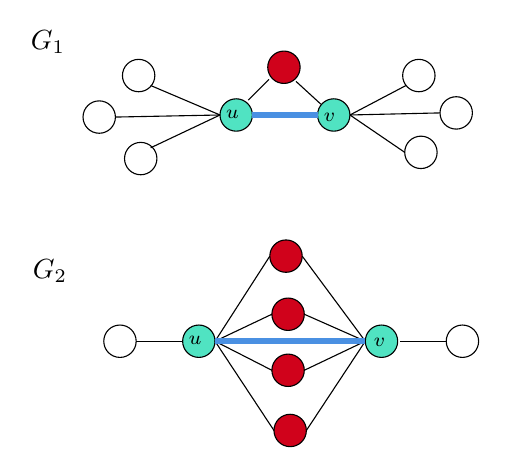
\begin{tikzpicture}[x=0.75pt,y=0.75pt,yscale=-1,xscale=1]
    %uncomment if require: \path (0,459); %set diagram left start at 0, and has height of 459
    
    %Shape: Circle [id:dp30741312121495734] 
    \draw  [fill={rgb, 255:red, 255; green, 255; blue, 255 }  ,fill opacity=1 ] (81.4,63.8) .. controls (81.4,59.49) and (84.89,56) .. (89.2,56) .. controls (93.51,56) and (97,59.49) .. (97,63.8) .. controls (97,68.11) and (93.51,71.6) .. (89.2,71.6) .. controls (84.89,71.6) and (81.4,68.11) .. (81.4,63.8) -- cycle ;
    %Shape: Circle [id:dp7121465720089162] 
    \draw  [fill={rgb, 255:red, 255; green, 255; blue, 255 }  ,fill opacity=1 ] (62.4,83.8) .. controls (62.4,79.49) and (65.89,76) .. (70.2,76) .. controls (74.51,76) and (78,79.49) .. (78,83.8) .. controls (78,88.11) and (74.51,91.6) .. (70.2,91.6) .. controls (65.89,91.6) and (62.4,88.11) .. (62.4,83.8) -- cycle ;
    %Shape: Circle [id:dp361848951371869] 
    \draw  [fill={rgb, 255:red, 255; green, 255; blue, 255 }  ,fill opacity=1 ] (82.4,103.8) .. controls (82.4,99.49) and (85.89,96) .. (90.2,96) .. controls (94.51,96) and (98,99.49) .. (98,103.8) .. controls (98,108.11) and (94.51,111.6) .. (90.2,111.6) .. controls (85.89,111.6) and (82.4,108.11) .. (82.4,103.8) -- cycle ;
    %Shape: Circle [id:dp9198149743646731] 
    \draw  [fill={rgb, 255:red, 255; green, 255; blue, 255 }  ,fill opacity=1 ] (216.4,63.8) .. controls (216.4,59.49) and (219.89,56) .. (224.2,56) .. controls (228.51,56) and (232,59.49) .. (232,63.8) .. controls (232,68.11) and (228.51,71.6) .. (224.2,71.6) .. controls (219.89,71.6) and (216.4,68.11) .. (216.4,63.8) -- cycle ;
    %Shape: Circle [id:dp9446452950264794] 
    \draw  [fill={rgb, 255:red, 255; green, 255; blue, 255 }  ,fill opacity=1 ] (234.4,81.8) .. controls (234.4,77.49) and (237.89,74) .. (242.2,74) .. controls (246.51,74) and (250,77.49) .. (250,81.8) .. controls (250,86.11) and (246.51,89.6) .. (242.2,89.6) .. controls (237.89,89.6) and (234.4,86.11) .. (234.4,81.8) -- cycle ;
    %Shape: Circle [id:dp993968354930985] 
    \draw  [fill={rgb, 255:red, 255; green, 255; blue, 255 }  ,fill opacity=1 ] (217.4,100.8) .. controls (217.4,96.49) and (220.89,93) .. (225.2,93) .. controls (229.51,93) and (233,96.49) .. (233,100.8) .. controls (233,105.11) and (229.51,108.6) .. (225.2,108.6) .. controls (220.89,108.6) and (217.4,105.11) .. (217.4,100.8) -- cycle ;
    %Shape: Circle [id:dp578563380682132] 
    \draw  [fill={rgb, 255:red, 80; green, 227; blue, 194 }  ,fill opacity=1 ] (128.4,82.8) .. controls (128.4,78.49) and (131.89,75) .. (136.2,75) .. controls (140.51,75) and (144,78.49) .. (144,82.8) .. controls (144,87.11) and (140.51,90.6) .. (136.2,90.6) .. controls (131.89,90.6) and (128.4,87.11) .. (128.4,82.8) -- cycle ;
    %Shape: Circle [id:dp9646589665089818] 
    \draw  [fill={rgb, 255:red, 80; green, 227; blue, 194 }  ,fill opacity=1 ] (175.4,82.8) .. controls (175.4,78.49) and (178.89,75) .. (183.2,75) .. controls (187.51,75) and (191,78.49) .. (191,82.8) .. controls (191,87.11) and (187.51,90.6) .. (183.2,90.6) .. controls (178.89,90.6) and (175.4,87.11) .. (175.4,82.8) -- cycle ;
    %Shape: Circle [id:dp9968177876122191] 
    \draw  [fill={rgb, 255:red, 208; green, 2; blue, 27 }  ,fill opacity=1 ] (151.4,59.8) .. controls (151.4,55.49) and (154.89,52) .. (159.2,52) .. controls (163.51,52) and (167,55.49) .. (167,59.8) .. controls (167,64.11) and (163.51,67.6) .. (159.2,67.6) .. controls (154.89,67.6) and (151.4,64.11) .. (151.4,59.8) -- cycle ;
    %Shape: Circle [id:dp42752465982325005] 
    \draw  [fill={rgb, 255:red, 208; green, 2; blue, 27 }  ,fill opacity=1 ] (154.4,234.8) .. controls (154.4,230.49) and (157.89,227) .. (162.2,227) .. controls (166.51,227) and (170,230.49) .. (170,234.8) .. controls (170,239.11) and (166.51,242.6) .. (162.2,242.6) .. controls (157.89,242.6) and (154.4,239.11) .. (154.4,234.8) -- cycle ;
    %Shape: Circle [id:dp15079474986730101] 
    \draw  [fill={rgb, 255:red, 208; green, 2; blue, 27 }  ,fill opacity=1 ] (152.4,150.8) .. controls (152.4,146.49) and (155.89,143) .. (160.2,143) .. controls (164.51,143) and (168,146.49) .. (168,150.8) .. controls (168,155.11) and (164.51,158.6) .. (160.2,158.6) .. controls (155.89,158.6) and (152.4,155.11) .. (152.4,150.8) -- cycle ;
    %Shape: Circle [id:dp7838455058284293] 
    \draw  [fill={rgb, 255:red, 208; green, 2; blue, 27 }  ,fill opacity=1 ] (153.4,178.8) .. controls (153.4,174.49) and (156.89,171) .. (161.2,171) .. controls (165.51,171) and (169,174.49) .. (169,178.8) .. controls (169,183.11) and (165.51,186.6) .. (161.2,186.6) .. controls (156.89,186.6) and (153.4,183.11) .. (153.4,178.8) -- cycle ;
    %Shape: Circle [id:dp9131805933832766] 
    \draw  [fill={rgb, 255:red, 208; green, 2; blue, 27 }  ,fill opacity=1 ] (153.4,205.8) .. controls (153.4,201.49) and (156.89,198) .. (161.2,198) .. controls (165.51,198) and (169,201.49) .. (169,205.8) .. controls (169,210.11) and (165.51,213.6) .. (161.2,213.6) .. controls (156.89,213.6) and (153.4,210.11) .. (153.4,205.8) -- cycle ;
    %Shape: Circle [id:dp24348081612151784] 
    \draw  [fill={rgb, 255:red, 80; green, 227; blue, 194 }  ,fill opacity=1 ] (110.4,191.8) .. controls (110.4,187.49) and (113.89,184) .. (118.2,184) .. controls (122.51,184) and (126,187.49) .. (126,191.8) .. controls (126,196.11) and (122.51,199.6) .. (118.2,199.6) .. controls (113.89,199.6) and (110.4,196.11) .. (110.4,191.8) -- cycle ;
    %Shape: Circle [id:dp12714206758934732] 
    \draw  [fill={rgb, 255:red, 80; green, 227; blue, 194 }  ,fill opacity=1 ] (198.4,191.8) .. controls (198.4,187.49) and (201.89,184) .. (206.2,184) .. controls (210.51,184) and (214,187.49) .. (214,191.8) .. controls (214,196.11) and (210.51,199.6) .. (206.2,199.6) .. controls (201.89,199.6) and (198.4,196.11) .. (198.4,191.8) -- cycle ;
    %Straight Lines [id:da14591538927994518] 
    \draw    (95,98.6) -- (128.4,82.8) ;
    %Straight Lines [id:da39552554089589886] 
    \draw    (95,68.6) -- (128.4,82.8) ;
    %Straight Lines [id:da20502375817106588] 
    \draw    (78,83.8) -- (128.4,82.8) ;
    %Straight Lines [id:da7939831218875366] 
    \draw [color={rgb, 255:red, 74; green, 144; blue, 226 }  ,draw opacity=1 ][line width=2.25]    (144,82.8) -- (175.4,82.8) ;
    %Straight Lines [id:da026131795551024295] 
    \draw    (191,82.8) -- (218,68.6) ;
    %Straight Lines [id:da2609512188985692] 
    \draw    (191,82.8) -- (234.4,81.8) ;
    %Straight Lines [id:da8084277469201291] 
    \draw    (191,82.8) -- (217.4,100.8) ;
    %Straight Lines [id:da10196698613186128] 
    \draw    (142,75.6) -- (152,65.6) ;
    %Straight Lines [id:da23311849914197968] 
    \draw    (165,66.6) -- (177,77.6) ;
    %Shape: Circle [id:dp11873261015665681] 
    \draw  [fill={rgb, 255:red, 255; green, 255; blue, 255 }  ,fill opacity=1 ] (72.4,191.8) .. controls (72.4,187.49) and (75.89,184) .. (80.2,184) .. controls (84.51,184) and (88,187.49) .. (88,191.8) .. controls (88,196.11) and (84.51,199.6) .. (80.2,199.6) .. controls (75.89,199.6) and (72.4,196.11) .. (72.4,191.8) -- cycle ;
    %Shape: Circle [id:dp33376506481092827] 
    \draw  [fill={rgb, 255:red, 255; green, 255; blue, 255 }  ,fill opacity=1 ] (237.4,191.8) .. controls (237.4,187.49) and (240.89,184) .. (245.2,184) .. controls (249.51,184) and (253,187.49) .. (253,191.8) .. controls (253,196.11) and (249.51,199.6) .. (245.2,199.6) .. controls (240.89,199.6) and (237.4,196.11) .. (237.4,191.8) -- cycle ;
    %Straight Lines [id:da2904263699945093] 
    \draw    (88,191.8) -- (110.4,191.8) ;
    %Straight Lines [id:da6780974128698207] 
    \draw    (215,191.8) -- (237.4,191.8) ;
    %Straight Lines [id:da6704766878520423] 
    \draw    (126,191.8) -- (152.4,150.8) ;
    %Straight Lines [id:da09171802499824078] 
    \draw    (126,191.8) -- (153.4,178.8) ;
    %Straight Lines [id:da11470962263923812] 
    \draw    (126,191.8) -- (153.4,205.8) ;
    %Straight Lines [id:da41877644456767915] 
    \draw    (126,191.8) -- (154.4,234.8) ;
    %Straight Lines [id:da7715077658766398] 
    \draw    (168,150.8) -- (198.4,191.8) ;
    %Straight Lines [id:da8383831101601573] 
    \draw    (169,178.8) -- (198.4,191.8) ;
    %Straight Lines [id:da8062049476940045] 
    \draw    (169,205.8) -- (198.4,191.8) ;
    %Straight Lines [id:da7386174273298884] 
    \draw    (170,234.8) -- (198.4,191.8) ;
    %Straight Lines [id:da4527673571237911] 
    \draw [color={rgb, 255:red, 74; green, 144; blue, 226 }  ,draw opacity=1 ][line width=2.25]    (126,191.8) -- (198.4,191.8) ;
    
    % Text Node
    \draw (130,79) node [anchor=north west][inner sep=0.75pt]  [font=\scriptsize] [align=left] {$\displaystyle u$};
    % Text Node
    \draw (177,80.6) node [anchor=north west][inner sep=0.75pt]  [font=\scriptsize] [align=left] {$\displaystyle v$};
    % Text Node
    \draw (201.2,189) node [anchor=north west][inner sep=0.75pt]  [font=\scriptsize] [align=left] {$\displaystyle v$};
    % Text Node
    \draw (112,188) node [anchor=north west][inner sep=0.75pt]  [font=\scriptsize] [align=left] {$\displaystyle u$};
    % Text Node
    \draw (36,41) node [anchor=north west][inner sep=0.75pt]    {$G_{1}$};
    % Text Node
    \draw (37,151) node [anchor=north west][inner sep=0.75pt]    {$G_{2}$};
    
    
    \end{tikzpicture}
    }%resizebox
    \caption{The set $N_{u}^{s} \cap N_{v}^{s}$ is in red, we assume that all $b_{e}^{rs} \leq 2$ for all $e$ the edges of $G_{1}$ and $G_{2}$. In the network at the top, we can see how the vertices $u$ and $v$ disperse their neighbors having a lower $ec_{(u,v)}^{\mathcal{G}}$ than in the figure below, where $u$ and $v$ integrate them, in terms of safety, it is important that the safest roads are integrated, otherwise, safety is seriously affected and reduced, as people will avoid traveling in a network that has safe roads dispersed through unsafe roads.}
    \label{Edge_clustering}
\end{figure}
%%%%%%%%%%%%%%%%%%%%%%%%%%%%%%%%%%%%%%%%%%%%%%%%%%%%%%%%%%%%%%%%%%%%%%%%%%%%%%%%




%%%%%%%%%%%%%%%%%%%%%%%%%%%%%%%%%%%%%%%%%%%%%%%%%%%%%%%%%%%%%%%%%%%%%%%%%%%%%%%%
\subsection{Degree Distribution (Intersection safety)}
\label{degree_distribution}

Given $v \in V$, its \textbf{degree} is defined as:
\begin{equation}
    k_{v} = \sum_{e \in A_{v}} w_{e}, \quad \textit{with } A_{v} \subset E \textup{ the set of adjacencies of } v.
\end{equation}
And through the degree, we can obtain the \textbf{degree distribution} by only plotting the nodes vs their degrees, which will give us a visual idea of how safe the network is on average. We can also observe, where the degrees of the vertices are skewed. In the case of obtaining a way to optimize the network, we can compare the difference of the areas obtained in the optimized case minus the original one. Otherwise, it is simply a visual way to observe the degrees of the network.
\begin{figure}
    \centering
    %\includegraphics[width=1.0\linewidth,height=1\textheight]
    \includegraphics[scale=0.4]{Images/centrality_degree.eps}
    \caption{Centrality degree}
    \label{Cd_academic_example}
\end{figure}

%-------------------------------------------------------------------------------

%%%%%%%%%%%%%%%%%%%%%%%%%%%%%%%%%%%%%%%%%%%%%%%%%%%%%%%%%%%%%%%%%%%%%%%%%%%%%%%%
\subsection{Eigenvector centrality}
This metric computes the importance of a node according to the importance of its neighbors and the importance of every one of its neighbors is determined by the importance of their respective neighbors and so on. Then a node with few important neighbors is considered more important than one with more neighbors less important. For our particular case, we are measuring how safe is an intersection according to the safety of its neighbors and the influence the safety of their neighbors on it, and so on. For this metric, we need the highest value, the safest. Then, for a node $v \in V$:
\begin{equation}
\label{eigen_cent}
    c_{E}(v) = \frac{1}{\lambda} \sum_{u \in N_{v}} \omega_{(u,v)}c_{E}(u),
\end{equation}
where $\lambda \in \mathbb{R}$ a constant, and $N_{v}$ is the set of neighbors of $v$. And with the help of the adjacency matrix $\mathbf{A}$, eq. \ref{eigen_cent} becomes as follows:
\begin{equation}
    c_{E}(v) = \frac{1}{\lambda} \sum_{u \in V} \mathbf{A}_{v,u} c_{E}(u), \, \forall v \in V,
\end{equation}
with $A_{v,u}$ the entry of the adjacency matrix $\mathbf{A}$ corresponding to the row of node $v$ and column of node $u$. And rewriting in matrix form:
\begin{equation}
\label{eigenvalue}
    \lambda \mathbf{c_{E}} = \mathbf{A} \mathbf{c_{E}},
\end{equation}
with $\mathbf{c_{E}}$ the vector where every entry corresponds to $c_{e}(v)$ for $v \in V$. And it is known that \ref{eigenvalue} is solved by finding the eigenvector $\mathbf{c_{E}}$ with eigenvalue $\lambda$. 
\begin{figure}
    \centering
    %\includegraphics[width=1.0\linewidth,height=1\textheight]
    \includegraphics[scale=0.4]{Images/eigenvevector_centrality.eps}
    \caption{Eigenvector centrality}
    \label{Eigenvector_centrality}
\end{figure}

%%%%%%%%%%%%%%%%%%%%%%%%%%%%%%%%%%%%%%%%%%%%%%%%%%%%%%%%%%%%%%%%%%%%%%%%%%%%%%%%
\section{Data}

%%%%%%%%%%%%%%%%%%%%%%%%%%%%%%%%%%%%%%%%%%%%%%%%%%%%%%%%%%%%%%%%%%%%%%%%%%%%%%%%
%%%%%%%%%%%%%%%%%%%%%%%%%%%%%%%%%%%%%%%%%%%%%%%%%%%%%%%%%%%%%%%%%%%%%%%%%%%%%%%%
%%%%%%%%%%%%%%%%%%%%%%%%%%%%%%%%%%%%%%%%%%%%%%%%%%%%%%%%%%%%%%%%%%%%%%%%%%%%%%%%
%%%%%%%%%%%%%%%%%%%%%%%%%%%%%%%%%%%%%%%%%%%%%%%%%%%%%%%%%%%%%%%%%%%%%%%%%%%%%%%%

\section{CONCLUSIONS}



\addtolength{\textheight}{-12cm}   % This command serves to balance the column lengths
                                  % on the last page of the document manually. It shortens
                                  % the textheight of the last page by a suitable amount.
                                  % This command does not take effect until the next page
                                  % so it should come on the page before the last. Make
                                  % sure that you do not shorten the textheight too much.

%%%%%%%%%%%%%%%%%%%%%%%%%%%%%%%%%%%%%%%%%%%%%%%%%%%%%%%%%%%%%%%%%%%%%%%%%%%%%%%%



%%%%%%%%%%%%%%%%%%%%%%%%%%%%%%%%%%%%%%%%%%%%%%%%%%%%%%%%%%%%%%%%%%%%%%%%%%%%%%%%



%%%%%%%%%%%%%%%%%%%%%%%%%%%%%%%%%%%%%%%%%%%%%%%%%%%%%%%%%%%%%%%%%%%%%%%%%%%%%%%%
\section*{APPENDIX}

%%%%%%%%%%%%%%%%%%%%%%%%%%%%%%%%%%%%%%%%%%%%%%%%%%%%%%%%%%%%%%%%%%%%%%%%%%%%%%%%

\subsection{Laplacian Spectral Theory? (\textbf{inverse brs})}
Let $n = |V|$, then the Laplacian $\mathcal{L} \in \mathbb{R}^{n \times n}$ of $\mathcal{G}$ is defined as follows:
\begin{equation}
\mathcal{L}_{ru,cv} = 
    \left\{\begin{matrix}
    1-\frac{b^{rs}(u,v)}{k_{u}} & \textup{ if } u=v \textup{ and } d_{u} \neq 0 \\ 
    -\frac{b^{rs}(u,v)}{\sqrt{k_{u} k_{v}}} & \textup{ if } (u,v) \in \mathcal{G} \\ 
    0 & \textup{ otherwise },
    \end{matrix}\right.
\end{equation}
where $r_{u}$ and $c_{v}$ is the index in a sorted list of $V$ with a given order of vertices $u$ and $v$ respectively. And $\forall v \in V \colon k_{v}$ is the degree of $v$, see subsection \ref{degree_distribution}. However, it does not seem to be a good metric in this specific case. see Fig. \ref{Laplacian}

%-------------------------------------------------------------------------------
\begin{figure}[h!]
\small
  \centering
  \begin{subfigure}[1_1]{0.3\linewidth}
    \includegraphics[width=\linewidth]{Images/laplacian_1.pdf}
     \caption{$\lambda_{1} \approx 0.714$}
  \end{subfigure}
  \begin{subfigure}[2_1]{0.3\linewidth}
    \includegraphics[width=\linewidth]{Images/laplacian_2.pdf}
    \caption{$\lambda_{1} \approx 0.507$}
  \end{subfigure}
  \begin{subfigure}[3_1]{0.3\linewidth}
    \includegraphics[width=\linewidth]{Images/laplacian_3.pdf}
    \caption{$\lambda_{1} \approx 0.771$}
  \end{subfigure}
  \caption{I found no pattern or sensitivity to increasing or decreasing edge security in that network, so I concluded that the second smallest eigenvalue is significant only in unweighted networks. The same was true when I tried to take into account the connectivity index $\chi(\mathcal{G}, \omega)$ \cite{araujo1998connectivity}}
  \label{Laplacian}
\end{figure}

\section*{ACKNOWLEDGMENT}





%%%%%%%%%%%%%%%%%%%%%%%%%%%%%%%%%%%%%%%%%%%%%%%%%%%%%%%%%%%%%%%%%%%%%%%%%%%%%%%%


%%%%%%%%%%%%%%%%%%%%%%%%%%%%%%%%%%%%%%%%%%%%%%%%%%%%%%%%%%%%%%%%%%%%%%%%%%%%%%%%

\bibliographystyle{IEEEtran}
\bibliography{IEEEabrv,mybibfile}







\end{document}
